\chapter{Immersive Environments: XR in Composition}
\label{ch:xr-mus}

%\textbf{Question three (Shahrokh Yadegari):} once a spatial work is created and recorded, what open XR technologies exist that one can leverage to present their works?

%What are the technical difficulties associated with this kind of work? What are the artistic difficulties associated with this kind of work? 

%What are the differences between WebXR, MobileXR and HMDs (or related technologies like CAVEs)? Be able to talk about the visual system in relation to XR.

%critical lens  
%This chapter will be developed with Shahrokh Yadegari. 

In this chapter we will discuss how open-source developments in XR are allowing more composers to experiment with spatial music and how these multi-sensory systems might be leveraged in the future for the dissemination of their music. We will also discuss some of the new compositional techniques that systems of this sort allow: non-linear sequences, interactivity in general, gamification of musical material, etc. 

We will address the different open source frameworks available for the development of these experiences and the technical, and artistic, difficulties associated with these works. We will describe in detail the most popular systems available today for the development of XR experiences and discuss the differences between them in terms of their affordances and limitations.

Namely, we will discuss outline the key trade-offs between presenting spatial music using: HMDs, CAVEs, in concert halls, in gallery spaces, or any other modalities that we might encounter. We are interested in open systems, and especially those that are accessible to those with limited resources (ie. people outside university settings). Finally, we will address some of the fundamental philosophical implications of these systems as they relate to the dichotomy between performer, composer, and audience. 

\section{Philosophy of Spatial Audio}

% In contemporary music settings, where artists rely on state-of-the-art tools for sound-making, we often forget how privileged we are to able to work in this domain, considering all the technological limitations faced by other artists. In this section we wanted to talk a bit about the philosophy of technology in art-making, and how open source solutions might address issues of equity. 

Technology has been an important part of art-making for many decades now. With the decreasing cost of computers, and their improved potential, more people today are capable of making art with computers than ever before. The technology industry remains focused on: improving, updating, and refining its products; in order to generate profit. Unfortunately, these systems are often designed with the latest hardware and operating systems in mind, which places an economic burden on composers and musicians. Furthermore, many popular exhibits and artistic works today feature technology as a core feature of the material, which excludes those who lack access or the skills to create such content.

Software, like digital art, poses a complex economic problem. Unlike physical objects, or direct services, software and digital art can easily be duplicated at little to no cost. Intellectual Property (IP) lies at the heart of this problem as was addressed by Puckette in \cite{puckette2004owns}. In his paper, Puckette used Pure Data (Pd) as a case study of what happens when a research institution commercializes its research. In the article, Puckette argues that IRCAM's\footnote{Institut de Recherche et Coordination Acoustique/Musique.} decision to enforce its IP claims to Pd and sell it as MAX/MSP resulted in a noted drop in the credibility of the institution as a research facility. The name Pd also means Public Domain. Drawing these IP lines is anything but simple since most valuable research draws from other authors' work. Similarly, most worthwhile artworks draw inspiration from its predecessors or contemporaries.

Much like software, digital art can be difficult to price. A physical painting can be analyzed to its authenticity and a price can be set based on what the market is willing to pay for it. A digital sound file, on the other hand, can be duplicated nearly for free, and mass distribution is just as cheap. A musical score operates on basically the same principle. \cite{puckette2001new} explored the idea of bringing some seminal computer music works into the public domain by using Pd, however, not all the works are included on his website, because IRCAM insisted some of patches be taken down. This creates an interesting dilemma for the composers, who naturally would prefer their music be performed as often as possible. 

When working in the scientific domain, one of the applied principles for validating experiments is the reproduction of the research. One of the benefits of using public domain tools, like Pd, is the ability to exercise a similar principle in the artistic domain. The idea being that aesthetic musical principles are hard to extend if the technology inherent to them is proprietary. In the pedagogical domain, this idea is also extremely powerful. Using public domain tools enables one to share their teachings with a wider subset of the population, without having to consider the economic barriers that software can sometimes create. 

Fernando Lopez-Lezcano, a composer and computer scientist at Stanford, has also been interested in this dichotomy for a long time. Fernando has been building Linux distributions for sound research at CCRMA for many years now. In \cite{CEC-eCon28-online} Fernando talks about the traditions established at Stanford related to open source software and how these have evolved over the years. 

%https://econtact.ca/11_3/index.html
%https://econtact.ca/11_3/lopez_lezcano_ccrma.html

\section{The History of VR}

Much before the first ever "real" VR experience was ever developed, pioneering painters, from as early as the 15th century, were already working on the concept of depth perception and optical perspective. Today we take for granted the idea that 2D representations of 3D space contain any dimensionality, but before the establishment of cameras, this was a feature which had to be creatively articulated by artists. The idea of a \textit{vanishing point}, the point at which receding parallel lines viewed in perspective appear to converge, shaped an entire generation of painters. Figure \ref{fig:san-pedro} shows Pietro Perugino's use of perspective in the "Entrega de las Llaves a San Pedro" fresco at the Sistine Chapel (1481–82).

Then, in 1878, one of the first examples of of \textit{stroboscopic apparent motion} was created by Eadward Muybridge\footnote{Muybridge was an English photographer important for his pioneering work in studies of photographic motion (9 April 1830 – 8 May 1904)}. This effect refers to the ability to generate apparent motion by flipping through a sequence of images at a fast rate. Figure \ref{fig:horse-motion} shows Muybridge's famous work "The Horse in Motion", depicting several "frames" of a horse as it seemingly moves across space. For this sequence 24 cameras were used, these were triggered by the horse as it moved along a track. In order to reproduce the images a \textit{zoopraxiscope}, also an invention of Muybridge, was used. The zoopraxiscope is a disc containing multiple image frames which is used to project a moving image in a recirculating fashion \cite{lavalle2016virtual}.

\begin{figure}[!htb]
\minipage{0.5\textwidth}
  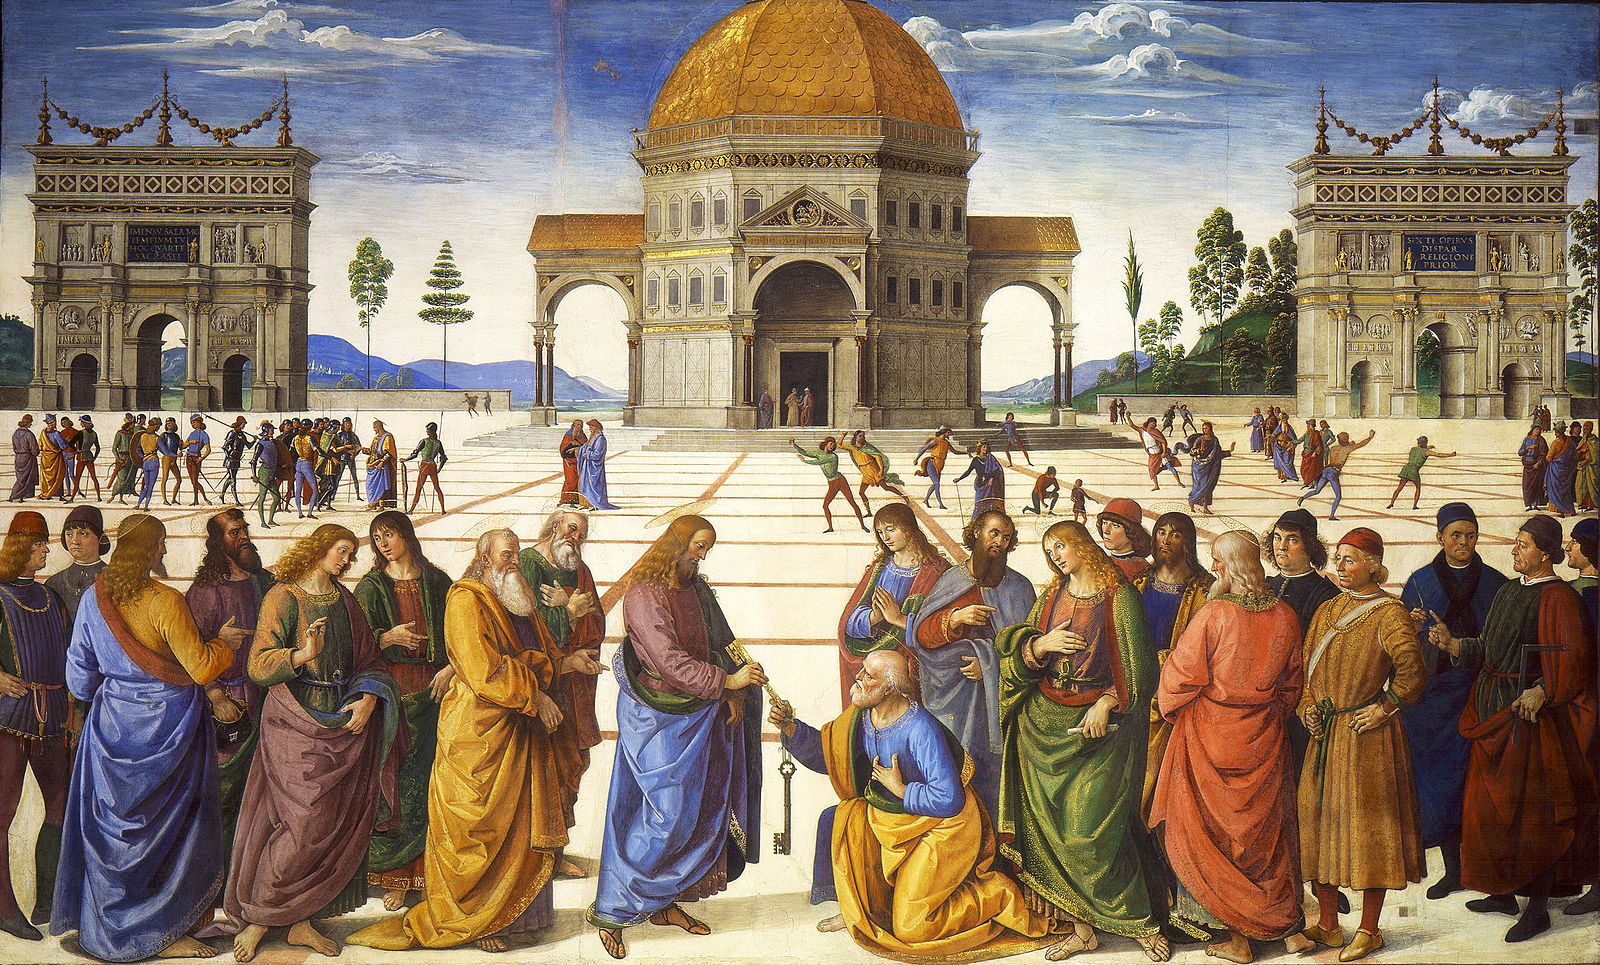
\includegraphics[width=\linewidth]{img/perugino.jpg}
  \caption{Entrega de las Llaves a San Pedro \cite{FileEntr24online}}\label{fig:san-pedro}
  % This work is in the public domain in its country of origin and other countries and areas where the copyright term is the author's life plus 100 years or fewer.
\endminipage\hfill
\minipage{0.5\textwidth}
  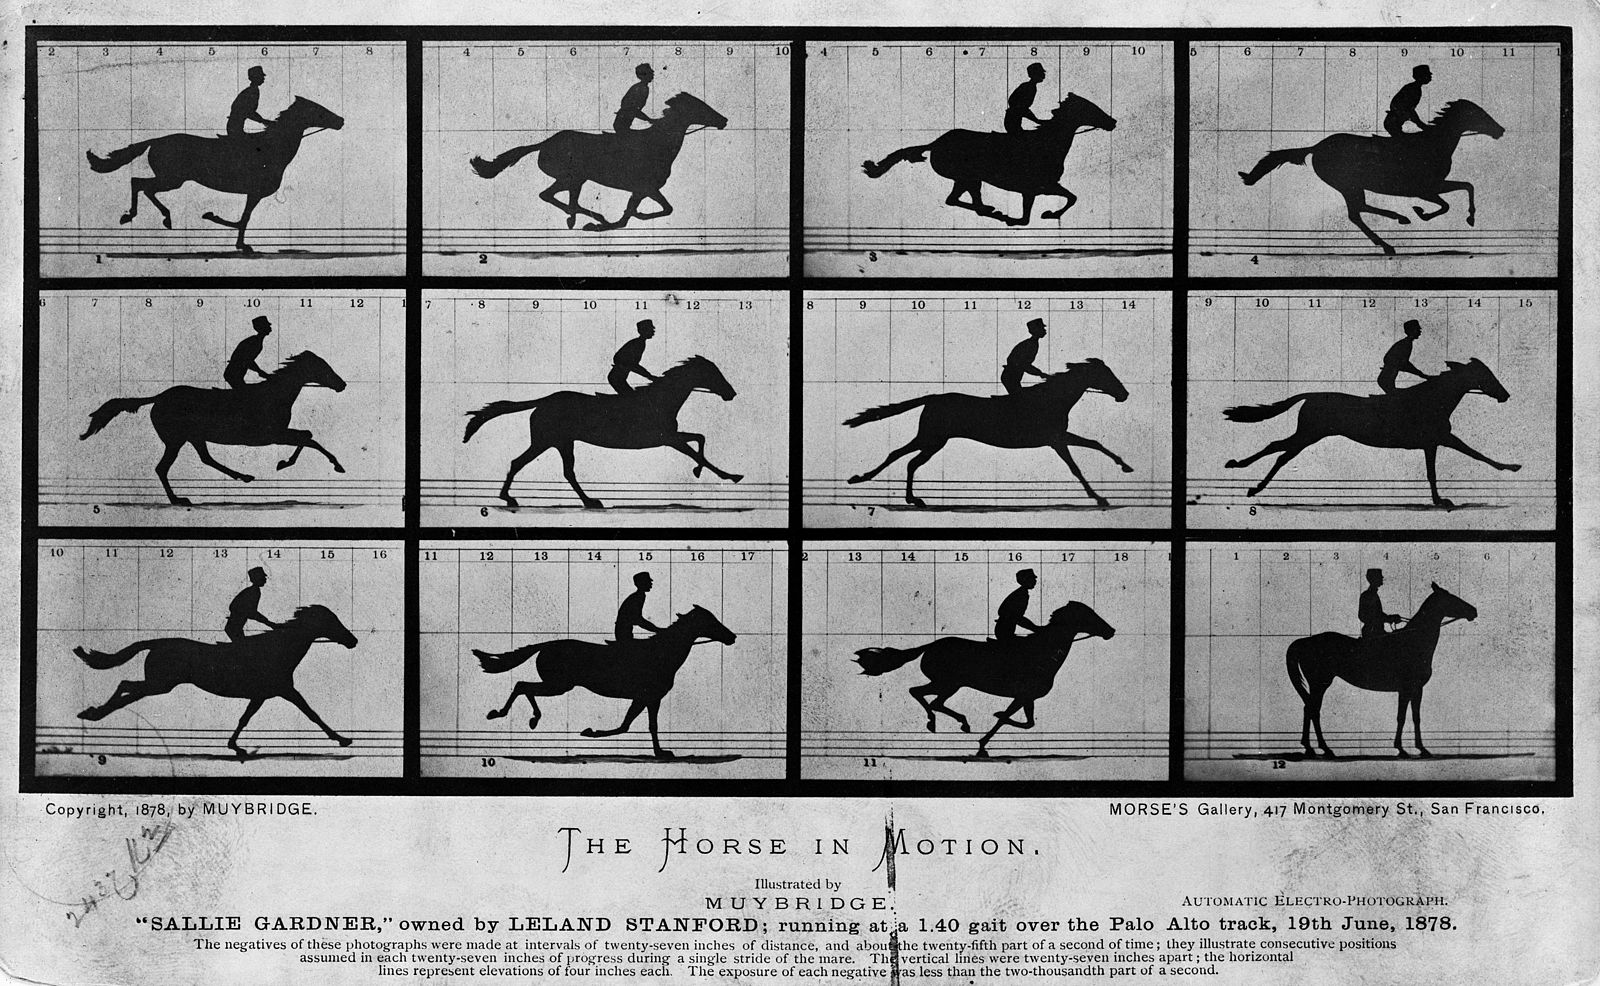
\includegraphics[width=\linewidth]{img/horse-in-mot.jpg}
  \caption{The Horse in Motion \cite{FileTheH64online}}\label{fig:horse-motion}
  % This work is in the public domain in the United States because it was published (or registered with the U.S. Copyright Office) before January 1, 1926.
\endminipage
\end{figure}

In 1838, the first stereoscope was invented by Charles Wheatstone \cite{hemstrom2020comparison}. A stereoscope is a device in which a pair of images is presented to each eye in order to provide the illusion of depth. By the 1930s, a portable version of a stereoscope called the View-Master became commercially successful. One of the innovations of this device was the increased field of view (FoV) and blocking of distracting boundary stimulus to increase immersion. In 1957, Morton Heilig introduced the Sensorama which added motion pictures, stereo sound, vibration, wind, and even smells in a personalized stereoscopic multi-modal experience. Unfortunately, the Sensorama had a fixed perspective, which meant the user was limited to a single orientation. It was also very large and expensive, which ultimately led to its downfall.

\begin{figure}[ht!]%force figure here, top, strict
\centering
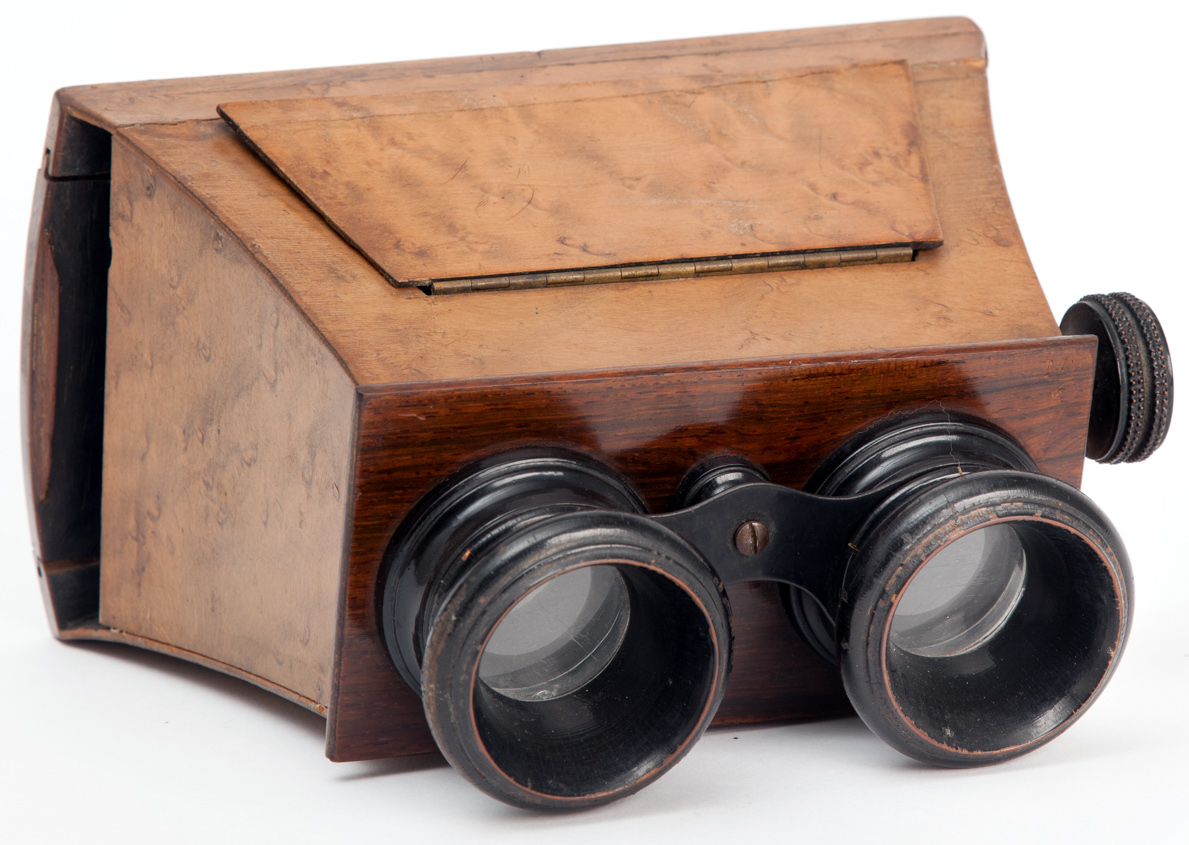
\includegraphics[width=0.7\textwidth]{img/stereoscope.jpg} 
%\captionsetup{justification=centering}
\caption{Brewster-type\protect\footnotemark stereoscope, 1870 \cite{FileIGB032online}}
\end{figure}

\footnotetext{Sir David Brewster (11 December 1781 – 10 February 1868) was a Scottish scientist, inventor, author, and academic administrator.}

Another well known method in film-making is \textit{3D movies} which are created using special cameras and then viewed using polarized light filters creating an additional sense of depth from a 2D image. Another way to increase immersion in films is to increase the FoV of the pictures by using a wider screen. The Cinerama is an example of such a system which used three projectors to extend the FoV and projected the image upon a concave surface for a richer viewing experience. It was created in the 1950s and is a precursor to the wide, curved, UltraWide LED (Light-Emitting Diode) monitors popular today. 

These two devices however, are not as immersive as the CAVE (Cave Automatic Virtual Environment) environments developed in 1992 at the University of Illinois. In these systems a larger number of projectors are used to, ideally, cover the entire surface of the room. Some CAVE systems also use 3D video in order to improve the depth perception of the image. The benefit of this approach is that the user does not need to wear any heavy equipment on their face which might restrict their ability to move. The downside is that such environments are often very costly to set-up given the large number of projectors needed to create the visual illusion. 

\subsection{Head-Mounted Displays}

In 1965, Ivan Sutherland introduce the concept of "The Ultimate Display", which he described as: "a room within which the computer can control the existence of matter." \cite{sutherland1965ultimate} A few years later, Sutherland and his team would build "The Sword of Damocles", regarded today as the first VR Head-Mounted Display (HMD).




\section{Contemporary XR Techniques}

LaValle defines VR in the introductory chapter of his book "Virtual Reality" \cite{lavalle2016virtual}: 

\begin{enumerate}
    \item \textbf{Targeted behavior:} The organism is having an “experience” that was designed by the creator. Examples include flying, walking, exploring, watching a movie, and socializing with other organisms.
    \item \textbf{Organism:} This could be you, someone else, or even another life form such as a fruit fly, cockroach, fish, rodent, or monkey (scientists have used VR technology on all of these!).
    \item \textbf{Artificial sensory stimulation:} Through the power of engineering, one or more senses of the organism become co-opted, at least partly, and their ordinary inputs are replaced or enhanced by artificial stimulation.
    \item \textbf{Awareness}: While having the experience, the organism seems unaware of the interference, thereby being “fooled” into feeling present in a virtual world. This unawareness leads to a sense of presence in an altered or alternative world. It is accepted as being natural.
\end{enumerate}

In contrast to Mixed Reality (MR) and Augmented Reality (AR), VR experiences completely block out real-world sensory stimuli. The key difference between MR and AR, is that AR experiences are passive while MR experiences allow the user to interact with the virtual world, and also allow the virtual world to interact with the real-world. 

For example, in a MR experience, an avatar that is displayed in your Field of View (FoV) might fall off a real table and respond to this event. In an AR experience we might see a simple overlay of time, temperature, and humidity on one's display. In these systems there are no apparent interactions between the real and virtual world. 

Unfortunately, these terms are quite loose today. It is more common for both consumers and companies to lump together AR and MR into a single category. It would appear that the typical consumer has become more familiar with the term AR, and a result it makes more financial sense to commercialize a MR using this alternate label. 

\subsection{Hardware}
Inn this section we will discuss some of the popular hardware solutions that exist for creation and reproduction of XR content. 

\subsubsection{HMDs}
Head mounted displays.
%https://scholar.google.com/scholar?hl=en&as_sdt=0%2C5&q=head-mounted+display+ieee&btnG=

\subsubsection{MOCAP}
MOtion CAPture systems. 
%https://arxiv.org/pdf/1607.02046.pdf

\subsubsection{360\textdegree cameras}
% https://ieeexplore.ieee.org/stamp/stamp.jsp?arnumber=7892229&casa_token=GSr2i72N1-cAAAAA:RmRLZa4onN2qE6AMEd_Hg_0m_JcehUXB1J28wL6PzpUA89UV3ZoNXvsUqlWV5ZNHG8tF-j8Lcuzn&tag=1

\subsubsection{CAVEs}
%https://www.sciencedirect.com/science/article/pii/S0167739X08001167?casa_token=pOdchEnz0b0AAAAA:_5pB4ufLKxGIrH6Si-_Z3cy31P9H2ZkxIUAHbYxPW26c4rvBZhCQVLYyDcUiBFL9Ug5TZHll5-Fc

\section{Software}
\subsection{Game Engines}
Unity, Unreal, Godot, etc.

\subsection{WebXR}
% https://immersive-web.github.io/webxr-samples/explainer.html
%https://www.khronos.org/gltf/

% Most usage of WebGL today happens via frameworks that significantly simplify the creation of 3D scenes compared to using raw WebGL. Some of the more popular examples are three.js, babylon.js, and PlayCanvas. There's also frameworks that are specifically designed to create XR content on the web, such as A-Frame and ReactVR. These are all fantastic libraries with their own strengths and focuses, and in general it's recommended that you find tools that suit your needs and rely on them rather than trying to build your own rendering systems from scratch.

% However, most frameworks will also hide away the details of interacting with the WebXR API. That's generally great for users, but not terribly useful when the entire point of your code is to demonstrate how to use the API! At the same time, we don't want the WebXR logic to be obscured by hundreds of lines of WebGL calls. As a result, these samples make use of their own minimalistic rendering library that is specifically designed to highlight use of the WebXR API and de-emphasize the WebGL rendering logic. It is not recommended that you use this library in your own projects, as you will almost certainly be better served by one of the more popular, better established frameworks.

\subsection{Mobile XR}
\section{Open XR Tools }
\section{The Future of XR}
\section{Conclusion}



